
\documentclass[a4paper,11pt]{article}

\usepackage{physics}
\usepackage{amsmath}
\usepackage{amssymb}
\usepackage{amsmath}
\usepackage{amsthm, mathtools}
%\usepackage{hyperref}
\usepackage{color}
\usepackage{jheppub}
\usepackage{tikz}
\usetikzlibrary{decorations.pathmorphing}
\usepackage[T1]{fontenc} % if needed

% My Documents
\newcommand{\be}{\begin{equation}}
\newcommand{\ee}{\end{equation}}
\newcommand{\bes}{\begin{equation*}}
\newcommand{\ees}{\end{equation*}}
\newcommand{\bea}{\begin{flalign*}}
\newcommand{\eea}{\end{flalign*}}


%\linespread{1.0}
%\setlength{\parindent}{0em}
%\setlength{\parskip}{0.8em}

\title{\textbf{AdS/CFT and Other Things}}
\author{Aditya Vijaykumar}
\affiliation{International Centre for Theoretical Sciences, Bengaluru, India.}
\emailAdd{aditya.vijaykumar@icts.res.in}
\abstract{This is one's effort to understand what the AdS/CFT Correspondence actually means, with explicit calculations and intuitive explanations of whatever is covered. In the course of one's journey, one hopes to review aspects of Quantum Field Theory as well as AdS spacetimes.
	
One shall mainly follow the path taken by Prof. Hong Liu in his MIT OCW course String Theory and Holographic Duality, supplementing it with one's own readings and observations. One shall also try to include as many references as possible.  }
\begin{document}
\maketitle
\section{Motivations}
From a field theory perspective, it is natural to ask whether a massless spin-$2$ particle \textcolor{red}{Ex : Why is gravity massless spin $ 2 $?} can arise as the bound state of a lower spin theory. If yes, that is equivalent to saying that gravity has effectively \textit{emerged}. Gluons and quarks can indeed form massive spin-$ 2 $ bound states which are unstable. \textcolor{red}{Ex : How do spin-$2$ particles arise in QCD?}.

But can one generate massless spin-$ 2 $ particles from this by maybe changing the theory a bit? Weinberg and Witten said no. They gave the following theorems

\begin{itemize}

\item \textbf{Theorem 1} - A theory that allows the construction of a Lorentz covariant conserved current cannot contain a massless particle of spin $  > 1/2 $ with non-vanishing charge.
\item \textbf{Theorem 2} - A theory that allows Lorentz covariant conserved stress tensor cannot contain massless particles of spin $ >1 $.
\end{itemize}
As GR need not have a conserved stress tensor \textcolor{red}{???}, these theorems do not forbid the graviton. But the second theorem also prohibits renormalizable theories in Minkowski spacetime in having an emergent gravity description. There is, however, a hidden assumption in this theory - it only applies to particles that live in the spacetime of the original theory. This seems like a straightforward, obvious assumption. But, in AdS/CFT, gravity lives in a different spacetime!

\textbf{\textcolor{red}{{Prove the Weinberg Witten Theorem}}}

\section{Black Holes ain't so Black}
In non-gravitational physics, in principle, one can probe arbitrarily large length scales. When gravity comes in, this stops being true. When $ E \gg m_p $, there will come a point when the Schwarzchild radius $ r_s \sim GE_{c} $ will become the fundamental distance scale. 

\subsection{Classical Black Holes}
The geometry outside the Schwarzschild Black Hole is given by,
\bes
ds^2 = -\qty(1-\frac{2M}{r})dt^2 + \qty(1-\frac{2M}{r})^{-1} dr^2 + r^2(d\theta^2 + \sin^2 \theta d\phi^2)
\ees
This has the following properties,
\begin{itemize}
	\item The solution is time reversal symmetric \textit{ie.} symmetric under $t \rightarrow -t$. Real black holes form through gravitational collapse, and hence this is not valid for them. Nonetheless, this can be assumed for late time black holes, which really makes the Schwarzschild solution a mathematical idealization of the actual black hole.
	\item Spacetime is non-singular at the horizon. Written in the Schwarzschild coordinates, the horizon is a coordinate singularity, and one can easily verify that it indeed is not a real singularity by \textcolor{red}{calculating curvature invariants}.
	\item $ r=r_s $ is a null hypersurface.
	\item The horizon is a surface of infinite redshift with respect to far away observer. \textcolor{red}{Show this explicitly}
	\item There are two important geometric quantities associated with the horizon,
	\bes
	\qq{Horizon Area} A_s = 4\pi r_s^2 = 16 \pi M^2 
	\ees
	\bes
	\qq{\textcolor{red}{Surface Gravity}} \kappa = \frac{1}{2}f'(r_s) = \frac{1}{2r_s} = \frac{1}{4M}
	\ees
		\centering
		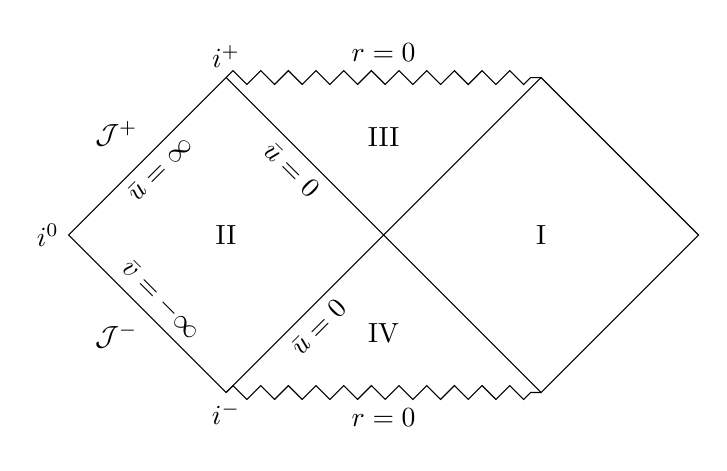
\begin{tikzpicture}[scale=0.5]
		\centering
		\node (I)    at ( 4,0)   {I};
		\node (II)   at (-4,0)   {II};
		\node (III)  at (0, 2.5) {III};
		\node (IV)   at (0,-2.5) {IV};
		
		\path  % Four corners of left diamond
		(II) +(90:4)  coordinate[label=90:$i^+$]  (IItop)
		+(-90:4) coordinate[label=-90:$i^-$] (IIbot)
		+(0:4)   coordinate                  (IIright)
		+(180:4) coordinate[label=180:$i^0$] (IIleft)
		;
		\draw (IIleft) -- 
		node[midway, above left]    {$\cal{J}^+$}
		node[midway, below, sloped] {$\bar{u}=\infty$}
		(IItop) --
		node[midway, below, sloped] {$\bar{u}=0$}
		(IIright) -- 
		node[midway, below, sloped] {$\bar{u}=0$}
		(IIbot) --
		node[midway, above, sloped] {$\bar{v}=-\infty$}
		node[midway, below left]    {$\cal{J}^-$}    
		(IIleft) -- cycle;
		
		\path % Four conners of the right diamond (no labels this time)
		(I) +(90:4)  coordinate (Itop)
		+(-90:4) coordinate (Ibot)
		+(180:4) coordinate (Ileft)
		+(0:4)   coordinate (Iright)
		;
		% No text this time in the next diagram
		\draw  (Ileft) -- (Itop) -- (Iright) -- (Ibot) -- (Ileft) -- cycle;
		
		% Squiggly lines
		\draw[decorate,decoration=zigzag] (IItop) -- (Itop)
		node[midway, above, inner sep=2mm] {$r=0$};
		
		\draw[decorate,decoration=zigzag] (IIbot) -- (Ibot)
		node[midway, below, inner sep=2mm] {$r=0$};
		
		\end{tikzpicture}
	
\end{itemize}
\end{document}